\documentclass[11pt,twoside]{scrartcl}
%\documentclass[11pt,twoside]{article}

%opening
\newcommand{\lecid}{15-316}
\newcommand{\leccourse}{Software Foundations of Security and Privacy}
\newcommand{\lecdate}{} %e.g. {October 21, 2013}
\newcommand{\lecnum}{8}
\newcommand{\lectitle}{Software Fault Isolation}
\newcommand{\lecturer}{Matt Fredrikson}
\newcommand{\lecurl}{https://15316-cmu.github.io/index}

\usepackage{varwidth}
\usepackage{lecnotes}
\usepackage[irlabel]{bugcatch}

\usepackage{tikz}
\usetikzlibrary{automata,shapes,positioning,matrix,shapes.callouts,decorations.text,patterns,trees,backgrounds}

% \usepackage[bracketinterpret,seqinfers,sidenotecalculus]{logic}
% \newcommand{\I}{\interpretation[const=I]}

% \newcommand{\bebecomes}{\mathrel{::=}}
% \newcommand{\alternative}{~|~}
% \newcommand{\asfml}{F}
% \newcommand{\bsfml}{G}
% \newcommand{\cusfml}{C}
% \def\leftrule{L}%
% \def\rightrule{R}%

\begin{document}

\newcommand{\atrace}{\sigma}%
%% the standard interpretation naming conventions
\newcommand{\stdI}{\dTLint[state=\omega]}%
\newcommand{\Ip}{\dTLint[trace=\atrace]}%
\newcommand{\ws}{\omega}\newcommand{\wt}{\nu}% 

\maketitle
\thispagestyle{empty}

%%%%%%%%%%%%%%%%%%%%%%%%%%%%%%%%%%%%%%%%%%%%%%

\section{Introduction \& Recap}

In the previous lecture we added memory to our language. We assume that the memory is just an array of values indexed by integers in the range $[0,\maxmem]$, and that it is undefined on any indices outside this range. Programs can read from memory by dereferencing it with the syntax $\pderef{\astrm}$, and update it with the syntax $\pumod{\pderef{\astrm}}{\bstrm}$.

We introduced axioms for reasoning about memory updates, being careful about bounds on accesses as necessary.
\begin{center}
\begin{calculus}
\cinferenceRule[mwrite|$\dibox{*}_{=}$]{mwrite}
{\linferenceRule[equiv]
  {p(\memupd{\pderefop}{\astrm}{\bstrm}) \land 0 \le \astrm < \maxmem}
  {\axkey{\dbox{\pderef{\astrm}:=\bstrm}{p(\pderefop)}}}
}{}%

\cinferenceRule[mreadeq|$\dibox{*}_{1}$]{mreadeq}
{\linferenceRule[sequent]
  {
    \lsequent{\Gamma}{\astrm=\astrm'}
    &\lsequent{\Gamma}{0 \le \astrm' < \maxmem}
  }
  {\lsequent{\Gamma}{\memupd{\pderefop}{\astrm}{\bstrm}(\astrm')=\bstrm}}
}{}%
\cinferenceRule[mreadneq|$\dibox{*}_{2}$]{mreadneq}
{\linferenceRule[sequent]
  {
    \lsequent{\Gamma}{\astrm\ne\astrm'}
    &\lsequent{\Gamma}{0 \le \astrm' < \maxmem}
  }
  {\lsequent{\Gamma}{\memupd{\pderefop}{\astrm}{\bstrm}(\astrm')=\pderef{\astrm'}}}
}{}%
\end{calculus}
\end{center}
We then defined memory safety for our language as the set of traces for which any terminal error state \errstate is not caused by a memory dereference or update. Using the axioms to prove safety covers most of memory safety as well, due to the bounds checks. But they don't cover dereferences that occur prior to updates, so if we want to ensure memory safety then we need to put assertions before each memory access that check to make sure its bounds are within $[0,\maxmem]$. Then proving any safety property for the resulting program will also be sufficient to demonstrate memory safety.

But what if we want to enforce a more granular type of memory safety policy to ensure that parts of our program don't read or write portions they aren't supposed to. This was motivated by our hypothetical career as an app developer who wants to monetize with advertising, and is thus compelled by Vladimir's discount ad shop to run untrusted rendering code within our program:
\[
\pif{\textit{display ads}}{\asprg}{\textit{continue without ads}}
\]
We discussed sandboxing policies where a region of memory is designated for the untrusted $\asprg$ to ``play'' in, such as the upper portion of memory at addresses 8-15 in the diagram below.
\begin{center}
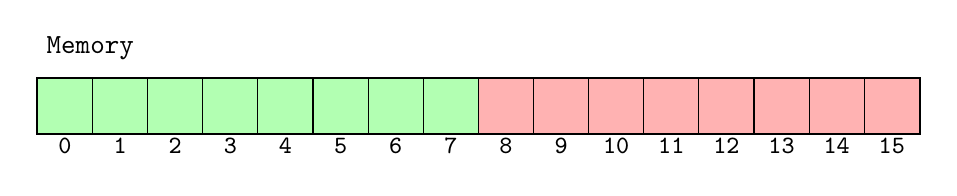
\begin{tikzpicture}[%
    arraynode/.style={
        draw,
        node contents={[\the\numexpr\pgfmatrixcurrentrow-2\relax][\the\numexpr\pgfmatrixcurrentcolumn-2\relax]},
        alias=n\the\numexpr\pgfmatrixcurrentrow-2\relax\the\numexpr\pgfmatrixcurrentcolumn-2\relax
        },
    columnlabel/.style={
        minimum size=0pt,
        draw=none,
        red,
        node contents={\the\numexpr\pgfmatrixcurrentcolumn-2\relax},
        alias=c\the\numexpr\pgfmatrixcurrentcolumn-2\relax
        },      
    rowlabel/.style={
        minimum size=0pt,
        draw=none,
        red,
        node contents={\the\numexpr\pgfmatrixcurrentrow-2\relax},
        alias=r\the\numexpr\pgfmatrixcurrentrow-2\relax
        },      
    emptynode/.style={node contents=~, draw=none},
    font=\ttfamily,
    array/.style={%
        matrix of nodes,
        nodes = arraynode,
        column sep=-\pgflinewidth,
        row sep=-\pgflinewidth, 
        nodes in empty cells,
        row 1/.style={nodes=columnlabel},
        column 1/.style={nodes=rowlabel},
        row 1 column 1/.style={%
            nodes=emptynode}}, 
    rowlabel2/.style={
        inner sep=2pt,
        draw=none,
        font=\small\ttfamily,
        node contents={\the\numexpr-1+\pgfmatrixcurrentcolumn\relax},
        alias=m\the\numexpr-1+\pgfmatrixcurrentcolumn\relax
        },      
    memoryrow/.style={%
        matrix of nodes,
        row 1/.style={nodes = {draw, minimum size=7mm}},
        column sep=-\pgflinewidth,
        row sep=-\pgflinewidth, 
        nodes in empty cells,
        row 2/.style={nodes=rowlabel2}}, 
    memory/.style={%
        matrix of nodes,
        nodes={draw, minimum size=6mm, anchor=center},
        row 1/.style={nodes = {columnlabel, black}},
        column 1/.style={nodes = {rowlabel, black}},
        row 1 column 1/.style={nodes = emptynode},
        column sep=-\pgflinewidth,
        row sep=-\pgflinewidth, 
        nodes in empty cells,
    } 
]

\begin{scope}[yshift=-4cm]

\matrix[memoryrow] (memrow) {
&&&&&&&&&&&&&&&\\
&&&&&&&&&&&&&&&\\};

\node[above right=1mm and 0 of memrow-1-1.north west] {Memory};
\draw[thick] (memrow-1-1.north west) rectangle (memrow-1-16.south east);

\begin{scope}[on background layer]
\fill[red!30] (memrow-1-9.north west) rectangle (memrow-1-16.south east);
\fill[green!30] (memrow-1-1.north west) rectangle (memrow-1-8.south east);
\end{scope}
\end{scope}

\end{tikzpicture}
\end{center}
As long as we can enforce this policy, and we are careful about writing our program to save and restore variable state, then we can ensure that whatever the sandbox does will not affect the rest of our program's execution.

We can certainly enforce such a policy by inserting $\passert{\ivr}$ commands before any memory read or write, to make sure that the indexed memory doesn't point outside the designated sandbox. But this approach has serious drawbacks. First, if $\asprg$ is simply buggy and makes accesses outside the sandbox, then the entire program will abort and our app will ``crash'' as far as the user is concerned. Second, Vladimir can actually force this outcome if he is maliciously inclined, and we certainly don't want to give such an attacker that kind of leeway.

Today we will discuss an approach called \emph{software fault isolation}~\cite{Sehr2010,Yee2009} (SFI) for properly isolating the malicious or buggy effects of $\asprg$ from the rest of our program. SFI works by inlining enforcement directly into $\asprg$, changing its behavior so that it can't violate the sandbox policy and if it attempts to do so then it still won't have any effect on the rest of our execution. SFI is a very practical technique, and has been used effectively in real applications to isolate untrusted code execution from browsers, operating systems, and other critical applications. In the next lab, you will implement a prototype SFI policy for your server.

Then we will look at a related technique called \emph{control flow integrity}~\cite{Abadi2009}, which ensures that the attacker cannot influence the control flow of a program to diverge from a pre-defined control flow policy. But in order for this defense to have any purpose, we need to introduce indirect control flow commands into our language, bringing it closer yet to the features that real platforms in need of rigorous security defenses have in practice.

\section{SFI: isolating sandbox policy violations}
Rather than checking whether memory accesses are safe and aborting if the check fails, perhaps we can force all untrusted accesses to be within the sandbox. In the diagram above, we use the specific sandbox policy $s_l=8, s_h=15$. Let us assume that our language operates over machine integers, so that the sandbox boundaries are the binary constants:
\[
s_l = \verb'0b1000', s_h = \verb'0b1111'
\]
So the range of valid sandbox addresses is \verb'0b1000', \verb'0b1001', \verb'0b1010', \ldots, \verb'0b1111'. 
Any valid address will have the fourth bit set to 1, and all greater bits set to 0. Given an arbitrary term $\astrm$, we can use bitwise operations to force it to a value in this range:
\begin{equation}
\label{eq:sfiex}
(\astrm \bitand \verb'0b1111') \bitor \verb'0b1000'
\end{equation}
What does this term accomplish? By first AND'ing the memory index $\astrm$ with \verb'0b1111', we ensure that none of the bits that are more significant than the fourth are set to 1.
This forces the term to be no greater than \verb'0b1111', or 15 in decimal.
By OR'ing this result with \verb'0b1000', we ensure that the bit in the fourth position is set to 1, which means that the result can be no less than $2^3 = 8$.
Thus, this term over the original index $\astrm$ has the effect of forcing accesses within the sandbox, 
\[
s_l = 8 \le (\astrm \bitand \verb'0b1111') \bitor \verb'0b1000' \le s_h = 15
\]
From now on, we will use hexadecimal rather than binary when writing such constants, so Equation~\ref{eq:sfiex} becomes $(\astrm \bitand \verb'0xF') \bitor \verb'0x8'$. If we assume that our sandbox regions always comprise integral boundaries (i.e., \verb'0x0000'-\verb'0x00FF', \verb'0x0100'-\verb'0x01FF', \verb'0x0200'-\verb'0x02FF'), then we can generalize this to:
\begin{equation}
\label{eq:sfiex}
(\astrm \bitand s_h) \bitor s_l
\end{equation}
With this in mind, we change the way we instrument programs.
\begin{itemize}
  \item Replace each command of the form $\pderef{\astrm}:=\bstrm$ with a new composed command:
  \[
  \pderef{(\astrm \bitand s_h) \bitor s_l}:=\bstrm
  \]
  This will ensure that $\asprg$ doesn't update any locations outside the sandbox.

  \item For any command $\bsprg$ containing the term $\pderef{\astrm}$, replace $\pderef{\astrm}$ with $\pderef{(\astrm \bitand s_h) \bitor s_l}$.
  This will ensure that $\asprg$ doesn't read any locations outside the sandbox.
\end{itemize}
This is called \emph{software fault isolation} (SFI).
The benefit of this approach is that as long as the sandbox is configured correctly for the memory, so that
\begin{equation}
0 \le s_l \le s_h < \maxmem
\end{equation}
Then after instrumenting the untrusted program $\asprg$, we know that \emph{(1)} it will not violate the sandbox safety policy, and \emph{(2)} it will also be memory safe! 

The semantics of the instrumented program will certainly differ from the original $\asprg$, in particular if it made unsafe memory accesses, and this may lead to bugs in the instrumented code that cause it to behave otherwise than expected. But this need not concern us, as our program will be completely isolated from the effect of these bugs, at least when it comes to the state of the memory.

\paragraph{Correctness of write instrumentation.} But how do we know that the instrumented program will actually satisfy the sandbox safety policy? Before when we used $\passert{\ivr}$ commands, we might have gotten away with an informal argument because the correctness was totally obvious. But now our instrumentation does strange things with bitwise operators to force certain behaviors. We should really be more formal about this to make sure we didn't screw things up.

The question becomes, how do we formalize the correctness of our sandbox policy as a safety property? Before we reasoned that the ``bad thing'' is a certain type of event, i.e. a read or write to memory locations outside the sandbox. We don't know how to prove things about these sorts of events, because all of the properties we have looked at so far define bad things  directly in terms of state. Perhaps we can think in terms of the effect that violations will have on program state instead of the events that bring those effects into being.

The first type of instrumentation purports to cover all write events. If $\asprg$ violates the policy by writing outside the sandbox, then the bad thing in terms of state would be that the contents of non-sandbox memory after $\asprg$ terminates differ from their contents prior to running $\asprg$. This sounds like something that we can formalize in dynamic logic using familiar properties, i.e. contracts.
\begin{equation}
\label{eq:sfi-integrity}
\forall i . \forall v . \lnot(s_l \le i \le s_h)  \land \pderef{i}=v \limply \dbox{\asprg}{\pderef{i}=v}
\end{equation}
But how can we prove this without knowing anything about what $\asprg$ is? We can reason inductively on the syntax of programs, which is what the proof of Theorem~\ref{thm:sfi-correctness} does.

\begin{theorem}
\label{thm:sfi-correctness}
Let $\asprg$ be a program whose memory update commands have been instrumented as prescribed by software fault isolation, and the sandbox low and high bounds are configured correctly, so that for all $x$:
\begin{equation}
\label{eq:bounds-assump}
0 \le s_l \le  (x \bitand s_h) \bitor s_l \le b_h < \maxmem
\end{equation}
Then all valid memory indices outside the sandbox retain the same value after executing $\asprg$ as they had prior to executing it. In other words, Equation~\ref{eq:sfi-integrity} is valid.
\end{theorem}
\begin{proof}
We will proceed by induction on the structure of $\asprg$. That is, we will show that for all of the simplest (base case) forms that $\asprg$ can take, the claim holds. Then we will use the inductive hypothesis for more complex forms of $\asprg$, showing that the claim holds whenever we assume that it does for any subprograms inside of $\asprg$. The inductive case thus covers all possible programs that can be constructed according to the syntax we introduced at the beginning of the lecture. This means that regardless of how $\asprg$ is implemented, the safety claim will hold.

The base cases of this proof correspond to programs that contain no other program constituents, i.e. $x:=\astrm$, $\pderef{\astrm}:=\bstrm$, and $\passert{\ivr}$. The inductive cases are programs that contain other programs, i.e. $\asprg;\bsprg$, $\pif{\ivr}{\asprg}{\bsprg}$, and $\pwhile{\ivr}{\asprg}$. We will complete the most challenging base case to outline the form of the proofs of the others, and leave the remaining ones as an exercise. We will do the same for one inductive case, leaving the rest as an exercise.

\paragraph{\textbf{Base case} $\pderef{\astrm}:=\bstrm$:} 
The instrumentation will replace this command with: 
\[
  \pderef{(\astrm \bitand s_h) \bitor s_l}:=\bstrm
\]
Then the following sequent derivation demonstrates correctness. Note that we use \irref{allr}, which is detailed in the aside at the end of these notes.
\begin{sequentdeduction}
\linfer[allr+allr] {
  \linfer[implyr+andl] {
    \linfer[mwrite] {
      \lsequent{\lnot(s_l \le i \le s_h), \pderef{i}=v}{\memupd{\pderefop}{(\astrm \bitand s_h) \bitor s_l}{\bstrm}(i)=v}
      &\ \lsequent{\ldots}{0 \le (\astrm \bitand s_h) \bitor s_l < \maxmem}
    } {
      \lsequent{\lnot(s_l \le i \le s_h), \pderef{i}=v}{\dbox{\pderef{(\astrm \bitand s_h) \bitor s_l}:=\bstrm}{\pderef{i}=v}}
    }
  } {
    \lsequent{}{\lnot(s_l \le i \le s_h)  \land \pderef{i}=v \limply \dbox{\pderef{(\astrm \bitand s_h) \bitor s_l}:=\bstrm}{\pderef{i}=v}}
  }
} {
  \lsequent{}{\forall i . \forall v . \lnot(s_l \le i \le s_h)  \land \pderef{i}=v \limply \dbox{\pderef{(\astrm \bitand s_h) \bitor s_l}:=\bstrm}{\pderef{i}=v}}
}
\end{sequentdeduction}
Note that in the above, the elided (\ldots) assumptions on the top-right branch are identical to those in the top-left branch.
They are left out only to ensure that the tree fits in the margins.

The right branch is left open, but we can discharge it from our assumption (\ref{eq:bounds-assump}) in the theorem statement.
At this point we need to split into cases on the left branch, because it could either be that $i = (\astrm \bitand s_h) \bitor s_l$ or $i \ne (\astrm \bitand s_h) \bitor s_l$. Depending on which case it is, we use \irref{mreadeq} or \irref{mreadneq}. We case split with the \irref{cut} rule. In the following, let
\[
P_1 \equiv i = (\astrm \bitand s_h) \bitor s_l, P_2 \equiv i \ne(\astrm \bitand s_h) \bitor s_l, P \equiv P_1 \lor P_2
\]
Then we continue with the proof as follows:
\begin{sequentdeduction}
\linfer[cut] {
  \linfer[qmear] {\lclose} {\lsequent{}{P}}
  &\ \ \linfer[orl] {
    \textcircled{1}
    &\textcircled{2}
  } {
    \lsequent{\lnot(s_l \le i \le s_h), \pderef{i}=v,P}{\memupd{\pderefop}{(\astrm \bitand s_h) \bitor s_l}{\bstrm}(i)=v}
    % \lsequent{\lnot(s_l \le i \le s_h), \pderef{i}=v_i,P}{Q}
  }
} {
  \lsequent{\lnot(s_l \le i \le s_h), \pderef{i}=v}{\memupd{\pderefop}{(\astrm \bitand s_h) \bitor s_l}{\bstrm}(i)=v}
}
\end{sequentdeduction}
The two remaining branches correspond to the cases where memory is dereferenced at the updated address $(\astrm \bitand s_h) \bitor s_l$ (\textcircled{1}), or anywhere else (\textcircled{2}).
Continuing with subtree \textcircled{1}:
\begin{sequentdeduction}
\linfer[notl] {
    \lsequent{\pderef{i}=v,i = (\astrm \bitand s_h) \bitor s_l}{s_l \le i \le s_h,\memupd{\pderefop}{(\astrm \bitand s_h) \bitor s_l}{\bstrm}(i)=v}
} {
  \lsequent{\lnot(s_l \le i \le s_h), \pderef{i}=v,i = (\astrm \bitand s_h) \bitor s_l}{\memupd{\pderefop}{(\astrm \bitand s_h) \bitor s_l}{\bstrm}(i)=v}
}
\end{sequentdeduction}
This part of the derivation asks us to prove that either $s_l \le i \le s_h$ or $\memupd{\pderefop}{(\astrm \bitand s_h) \bitor s_l}{\bstrm}(i)=v$, from the assumptions that $\pderef{i}=v$ and $i = (\astrm \bitand s_h) \bitor s_l$. Let's think about the cases a bit.
\begin{itemize}
\item We could try to prove that $\memupd{\pderefop}{(\astrm \bitand s_h) \bitor s_l}{\bstrm}(i)=v$. At first glance this might seem promising, because of the assumption that $\pderef{i}=v$. But we also assume that $i = (\astrm \bitand s_h) \bitor s_l$, and \irref{mreadeq} tells us then that $\memupd{\pderefop}{(\astrm \bitand s_h) \bitor s_l}{\bstrm}(i) = \bstrm$. We don't have an assumption which says that $v = \bstrm$, which we would need to do the proof this way.
\item We can alternately prove that $s_l \le i \le s_h$. We have in our context that $i = (\astrm \bitand s_h) \bitor s_l$, and the theorem assumes (\ref{eq:bounds-assump}) which gives us an even stronger property $0 \le s_l \le  (x \bitand s_h) \bitor s_l \le b_h < \maxmem$. We can invoke \irref{qmear} to discharge the obligation:
\[
0 \le s_l \le  (x \bitand s_h) \bitor s_l \le b_h < \maxmem \limply s_l \le i \le s_h
\]
We complete the proof of subtree \textcircled{1} this way, and can move on with the proof.
\end{itemize}

Now we complete this case of the proof by deriving \textcircled{2}.
Note that we begin by applying the \irref{weakenl} rule, which removes some unneeded assumptions from our context and makes the proof more concise.
\[
\cinferenceRule[weakenl|W\leftrule]{left weakening}
{\linferenceRule[sequent]
  {\lsequent[L]{}{}}
  {\lsequent[L]{\asfml}{}}
}{}%
\]
This rule is perfectly sound, which you can verify yourself as a proof exercise.
\begin{sequentdeduction}
\linfer[weakenl] {
  \linfer[cut] {
    \linfer[mreadneq] {
      \linfer[id]{\lclose}{\lsequent{\pderef{i}=v,i \ne (\astrm \bitand s_h) \bitor s_l}{i \ne (\astrm \bitand s_h) \bitor s_l}}
      &\lsequent{\pderef{i}=v,i \ne (\astrm \bitand s_h) \bitor s_l}{0 \le i < \maxmem}
    } {
      \lsequent{\pderef{i}=v,i \ne (\astrm \bitand s_h) \bitor s_l}{\memupd{\pderefop}{(\astrm \bitand s_h) \bitor s_l}{\bstrm}(i)=\pderef{i}}
    }
  } {
    \lsequent{\pderef{i}=v,i \ne (\astrm \bitand s_h) \bitor s_l}{\memupd{\pderefop}{(\astrm \bitand s_h) \bitor s_l}{\bstrm}(i)=v}
  }
} {
  \lsequent{\lnot(s_l \le i \le s_h), \pderef{i}=v,i \ne (\astrm \bitand s_h) \bitor s_l}{\memupd{\pderefop}{(\astrm \bitand s_h) \bitor s_l}{\bstrm}(i)=v}
}
\end{sequentdeduction}
The unfinished portion of the proof assumes that $\pderef{i}=v$ and $i \ne (\astrm \bitand s_h) \bitor s_l$ imply that $0 \le i < \maxmem$. Recall that memory dereferences are undefined whenever the index is out of bounds, and our assumption is that the memory at index $i$ \emph{is} in fact defined, and takes the value $v$. From this we conclude that $i$ must be in bounds. This completes the base case for memory updates.

\paragraph{Inductive case $\asprg;\bsprg$:}
Suppose that the program is a composition of $\asprg$ and $\bsprg$. The inductive hypothesis lets us assume that:
\begin{align}
\label{eq:a1}
\forall i . \lnot(s_l \le i \le s_h)  \land \pderef{i}=v &\limply \dbox{\asprg}{\pderef{i}=v} \\
\label{eq:a2}
\forall i . \lnot(s_l \le i \le s_h)  \land \pderef{i}=v &\limply \dbox{\bsprg}{\pderef{i}=v}
\end{align}
Then consider $(\omega,\ldots,\mu) \in \llbracket\asprg\rrbracket$ and $(\mu,\ldots,\nu) \in \llbracket\bsprg\rrbracket$. We have the following which says that the memory outside the sandbox in the initial state remains unchanged until the final state, for both $\asprg$ and $\bsprg$:
\begin{align}
\label{eq:trans1}
\forall i . \lnot(s_l \le i \le s_h)  \land \omega_M(i)=v &\limply \mu_M(i)=v \\
\label{eq:trans2}
\forall i . \lnot(s_l \le i \le s_h)  \land \mu_M(i)=v &\limply \nu_M(i)=v
\end{align}
This follows directly from the semantics of $\pderef{i}$, which refer to the memory component of states $\omega, \mu,$ and $\nu$, and the box modalities in (\ref{eq:a1}) and (\ref{eq:a2}).

Notice that the right side of the implication in (\ref{eq:trans1}) matches up with the latter half of the conjunction in the left side of the implication in (\ref{eq:trans2}).
From this and the semantics of $\asprg;\bsprg$, it must then be that for all $(\omega,\ldots,\nu)\in\llbracket\asprg;\bsprg\rrbracket$ we can say:
\begin{equation}
\label{eq:transc}
\forall i . \lnot(s_l \le i \le s_h)  \land \omega_M(i)=v \limply \nu_M(i)=v
\end{equation}
Then (\ref{eq:transc}) and the semantics of the box modality with $\asprg;\bsprg$ tell us that 
\begin{equation}
\forall i . \lnot(s_l \le i \le s_h)  \land \pderef{i}=v \limply \dbox{\asprg;\bsprg}{\pderef{i}=v}
\end{equation}
This completes the inductive case for composition. 
% In the following let $P \equiv \lnot(s_l \le i \le s_h),\pderef{i}=v_i$.
% \begin{sequentdeduction}
% \linfer[allr+implyr+andl+composeb] {
%   \linfer[notl] {
%     \linfer[Mbr] {
%       \lsequent{\pderef{i}=v_i}{\dbox{\asprg}{\pderef{i}=v_i},s_l \le i \le s_h}
%       &\lsequent{\lnot(s_l \le i \le s_h),\pderef{i}=v_i}{\dbox{\bsprg}{\pderef{i}=v_i}}
%     } {
%       \lsequent{\pderef{i}=v_i}{\dibox{\asprg}\dbox{\bsprg}{\pderef{i}=v_i},s_l \le i \le s_h}
%     }
%   } {
%     \lsequent{\lnot(s_l \le i \le s_h),\pderef{i}=v_i}{\dibox{\asprg}\dbox{\bsprg}{\pderef{i}=v_i}}
%   }
% } {
%   \lsequent{}{\forall i . \lnot(s_l \le i \le s_h)  \land \pderef{i}=v_i \limply \dbox{\asprg;\bsprg}{\pderef{i}=v_i}}
% }
% \end{sequentdeduction}

\paragraph{Rest of the proof:}
The remaining cases are left as exercises. The remaining base cases should be relatively straightforward to complete, because they correspond to program forms that do not affect the memory state at all. The inductive cases follow the form outlined for $\asprg;\bsprg$ above, using the inductive hypothesis as well as the semantics of programs and dynamic logic to conclude that whenever subprograms satisfy the sandbox policy, the larger programs that contain them do as well.
\end{proof}
So we have now concluded that software fault isolation prevents memory write operations from working outside the designated sandbox. What about read operations? The second form of instrumentation is applied to terms that read from the current memory state, and we expect that they will prevent programs from unauthorized reads for the same reasons that write operations are safe.

\paragraph{Correctness of read instrumentation.}
We based our proof of write operations on the fact that it can be formalized as a safety property over program state. We reasoned that if the instrumentation were not sufficient, then there would be evidence at the end of $\asprg$'s execution in the form of memory contents that were modified from their initial value. But can we say something similar about memory read operations? What evidence in the state will there be if the instrumentation is not correct, and $\asprg$ succeeds at reading a memory location outside the sandbox?

We might say that if there was a successful read outside the sandbox, then one of the program variables, or perhaps one of the sandbox memory cells, will contain a value that was initially in the memory outside the sandbox. But this need not be the case, because what if $\asprg$ makes an unauthorized read, and then performs an operation in the result before storing it in a variable or memory? On the other hand, suppose that in $\asprg$'s final state, one of the variables \emph{did} take the same value as an unauthorized memory location. Are we certain that it took this value because of an unauthorized read, or could it be mere chance the $\asprg$ happened to compute a value that overlapped with outside memory?

This question drives to a fundamental difference between safety and information flow properties. We've learned that safety properties can be viewed as collections of traces, so all that we need to do to reason about whether a program satisfies such a property is make sure all of its traces are in the property. This is what SFI accomplishes when it forces memory accesses to a particular range, because the property says that all traces must only make accesses within that range. Likewise, this is what we prove when we use dynamic logic sequent calculus deductions to reason about safety: that all terminating traces are in the set described by the property.

But information flow properties are fundamentally different. They cannot be described as sets of traces, and in fact must consider what \emph{might} have happened on a different trace if some variable or memory location had taken a different value. To reason convincingly about the correctness of the read operations we need to be able to refer to and prove things about information flow properties, i.e. that information outside the sandbox does not flow into any of the variables or memory locations within the sandbox. This will be a topic of future lectures, where we will take a completely different approach to policy enforcement.

\begin{figure}
\fbox{
\begin{minipage}{\textwidth}
\textbf{Aside}: Rules for quantifiers
\\[1ex]
Our proof of SFI correctness used a rule that we have not seen before: $\forall\rightrule$. The rule allows us to remove the quantifier, replacing the bound variable with a new variable that does not appear anywhere else in the sequent. This is equivalent to saying that if we can prove that $F(y)$ holds on some $y$ for which we make no prior assumptions, then we can conclude that it holds universally. The corresponding left rule ($\forall\leftrule$) says that if we can prove something assuming $F$ holds for a particular term, say $\astrm$, then we can prove it assuming that $F$ holds universally. Intuitively, we've only made our assumptions stronger by assuming that $F$ holds universally.
\[
\cinferenceRule[allr|$\forall$\leftrule]{forall left}
{\linferenceRule[sequent]
  {\lsequent{\Gamma,F(\astrm)}{{}\Delta}}
  {\lsequent{\Gamma,\forall x.F(x)}{{}\Delta}}
}{}
\quad
\cinferenceRule[allr|$\forall$\rightrule]{forall right}
{\linferenceRule[sequent]
  {\lsequent{\Gamma}{{}F(y),\Delta}}
  {\lsequent{\Gamma}{{}\forall x.F(x),\Delta}}
}{\text{$y$ new}}
\]
The rules for existential quantifiers are similar, but in this case, it is the left rule in which we need to be careful about renaming. Similarly to the $\forall\rightrule$, if we can use the fact that $F(y)$ holds to prove $\Delta$, and nothing in our assumptions or $\Delta$ mentions specific things about $y$, then we can conclude that the details of $y$ don't matter for the conclusion, and the only important fact is that some value establishing $F(y)$ exists. The $\exists\rightrule$ simply says that if we can prove that $F$ holds for term $\astrm$, then we can conclude that it must hold for some value, even if we leave the value unspecified.
\[
\cinferenceRule[existsr|$\exists$\leftrule]{exists left}
{\linferenceRule[sequent]
  {\lsequent{\Gamma,F(y)}{{}\Delta}}
  {\lsequent{\Gamma,\exists x.F(x)}{{}\Delta}}
}{\text{$y$ new}}
\quad
\cinferenceRule[existsr|$\exists$\rightrule]{exists right}
{\linferenceRule[sequent]
  {\lsequent{\Gamma}{{}F(\astrm),\Delta}}
  {\lsequent{\Gamma}{{}\exists x.F(x),\Delta}}
}{}
\]
\end{minipage}
}
\end{figure}

% \bibliographystyle{abbrv}
\bibliography{bibliography}
\end{document}